%\section{L1 Minimization via Interior Point Method} % TODO

\subsection{Introduction} 
% 
In this section we are interested in deriving efficient numerical methods
for solving the following optimization problem:  Given a set of $n$
non-negative piecewise smooth functions $a_j(\u)$ and a non-negative piecewise
smooth function $y(\u)$,  find a linear combination of $a_j(\u)$ parameterized
by $\x \in \Re^n$ that minimizes the absolute value of the error function
$e(\u) = \sum_ja_j(\u) x_j - y(\u)$, integrated over some compact domain $U$.

In the context of illumination invariant face recognition, $a_j$ are a database
of images of one person's face under different illuminations, and $y$ is
another image of a (possibly different) person's face.  In this case, $\u \in
\Re^2$ is the 2D image coordinate, and $U$ is a mask that includes a subset of
the human face.  In this case, the minimization problem becomes:
\begin{equation}
\label{eqn:continuous2D} 
\tilde{\x} = \argmin{\x\in \Re^n} \iint_U{\left|\left(\sum_{j=1,\ldots,n} a_j(\u) x_j\right) - y(\u)\right| du_1 du_2} 
\end{equation}

For the sake of discussion, we will focus on the simplified case where $a_i$
are piecewise smooth function of a scalar valued $u$.  Note that if we
discretize an image with respect to one of the image coordinates and
concatenate the resulting functions, we are left with a new function that is
still piecewise continuous.  This fact may turn out useful in practice; it may
be possible to make use of the piecewise smoothness of our original function in
one direction while ignoring its additional smoothess in the other direction.
Under this reduction we are left with the following minimization:
\begin{equation}\label{eqn:continuous1D}
\tilde{\x} = \argmin{\x\in \Re^n} \int_U{ \left|\left(\sum_{j=1,\ldots,n} a_j(u) x_j\right) - y(u)\right| du}
\end{equation}

For notational convenience, we will further define symbols:
\begin{equation}
 f(x) = \int_U{ \left|\left(\sum_{j=1,\ldots,n} a_j(u) x_j\right) - y(u)\right| du}
\end{equation}
is the cost function we are trying to minimize.
\begin{equation}
 e(x,u) = \left|\left(\sum_{j=1,\ldots,n} a_j(u) x_j\right) - y(u)\right| du
\end{equation}
is our error function.

{\bf Convexity of $f$ in the Continuous Case } 
%
It is easy to show that $f(\x)$
is a convex function in the continuous case.  To do this, it is sufficient to
show that:
%
\begin{eqnarray*}
f(\alpha \x^- + (1-\alpha) \x^+) 
	&\leq& \alpha f(\x^-) + (1-\alpha) f(\x^+) \\
\int \left|\sum_j a_j (\alpha x_j^- + (1-\alpha) x_j^+) - y\right| du 
	&\leq& \alpha \int \left|\sum_j a_j x_j^- - y\right|du + (1 - \alpha) \int \left|\sum_j a_j x_j^+ - y\right|du
\end{eqnarray*}
%
If we move the $\alpha$ and $(1-\alpha)$ inside the integrals and into the absolute values, 
and drop the integrals, we find that it it sufficient to show that:
%
\begin{equation*}
\left|\sum_j a_j (\alpha x_j^- + (1-\alpha) x_j^+) - y\right|
	\leq \left|\sum_j a_j (\alpha x_j^-) - \alpha y\right| + \left|\sum_j a_j (1 - \alpha) x_j^+ - (1 - \alpha) y\right|.
\end{equation*}
%
The terms inside the left absolute value are the exact same terms 
that are found inside the right two absolute values, so the inequality holds, and $f$ is convex. 

As a first step towards designing an efficient numerical algorithms for
minimizing the function f, we must choose a method of evaluating the integral
numerically.  One common way to do this is to choose an interpolation function
that is easier to integrate, but still closely approximates the original
function.  One way to do this is to chose an interpolating function that
matches the original function exactly at a uniformly spaced set of sampling
points, and interpolates between them.  The two we will be most interested in
are the rectangle rule and the trapezoidal rule.  

Since we are interested in the effect of the absolute value on the value of f,
we will choose to approximate it as an integral of the absolute value of the
weighted sums of interpolated versions of $a_j$ and $y$, rather than computing
it as an integral of an interpolated version of $|e|$.  This better models the
original integral, since sign changes in $e$ will typically occur between
sample points.  Furthermore, since $f$ is convex in general, we will not break
the convexity of our optimization problem by substituting in approximate
versions of $a_j(u)$ and $y(u)$.  We will be concerned with what effect the
choice of approximating functions will have on the derivatives of $f$ with
respect to $x$.

\section{Geometry of the $\ell_1$ representation problem}
{\bf Rectangle Rule} 
%
The rectangle rule for numerical integration implements an
integral as the integral of a piecewise constant approximation of the original
function.  The approximating function matches the original at samples located
at the midpoints of the sampling regions. This is illustrated in figure
\ref{fig:rectangle}.
%
\begin{figure}
 \centering
 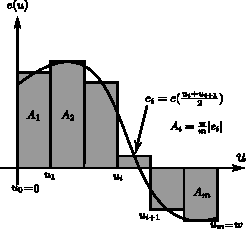
\includegraphics[width=3in]{figures_subgradient/integration_rectangle_midpoint.pdf}
 % integration_rectangle_midpoint.pdf: 119x111 pixel, 72dpi, 4.20x3.92 cm, bb=0 0 119 111
 \caption{Numerical integration of a function $e(u)$ by the Rectangle Rule for 1D $u$.}
 \label{fig:rectangle}
\end{figure}
%
The figure shows this approximation as applied to $e(u)$. The values $e_i$ serve as the parameterization of the surrogate function and are samples of the original function $e(u)$, and can be stacked up into a vector $\e$.  Using the fact that the sum of two parameterized functions is parametized by the sum of their parameters, we can easily compute a numerical approximation to our objective function as:
%
\begin{equation}\label{eqn:discrete1DBox}
f_r = \frac{w}{m} \sum{ \left|\left(\sum_{j=1,\ldots,n} \a_j x_j\right) - \y\right|}
\end{equation}
%
where $\a_j, \y \in \Re^m$ are vectors containing the sampled values of $a(u)$ and $y(u)$.  If we pack $\a_j$ into the columns of a matrix $A \in \Re^{m \times n}$, we are left with the the familiar expression:
%
\begin{equation}
\label{eqn:original_formulation}
\tilde{\x_r} = \argmin{\x\in \Re^n} \frac{w}{m} || A \x - \y ||_1
\end{equation}
%
Note that in the recognition step of the face recognition application, it is necessary to 
perform a minimization of the form:
%
\begin{equation}
\label{eqn:recognition_formulation}
\tilde{\x_r} = \argmin{\x\in \Re^n} \frac{w}{m} || A \x - \y ||_1 + ||\x||_1
\end{equation}
%
Note that the optimization problem formulation \ref{eqn:recognition_formulation} can
be converted to the formulation \ref{eqn:original_formulation} by appending an identity
matrix to the bottom of $A$ and zeros to the bottom of $\y$.  For very tall $A$,
doing so will not greatly affect the dimension of the problem, so it may not even
be necessary to take advantage of the special structure of the 
(relatively small) identity matrix in numerical implementation.

{\bf Geometry of the optimization problem for Rectangle Rule}  
%
In understanding
the behavior of iterative optimization routines, it will be instructive to
build a picture of the objective function $f$ in our heads.  
If we let $\a_i$
be the rows of $A$ from \ref{eqn:original_formulation}, the objective function
can be expressed as:
\begin{equation}
f_r = \sum_{i=1\ldots m}| \a_i \x - y_i | = \sum_{i=1\ldots m} |e_i|
\end{equation}
Each $e_i$ is a linear function of $x$. It has a gradient $\a_i$ in the
positive orthant and has been shifted ``downwards'' by $y_i$.  If $n=2$ we can
plot the $|e_i|$ as a function of $x_1$ and $x_2$.  It will look like a trough
that touches zero at the line $\a_i \x - y_i=0$.  $f$ will be the sum of $m$
such troughs, and thus will be convex, continuous, and piecewise linear with
gradient discontinuities at the hyperplanes defined by $\a_i \x - y_i=0$.
Intuitively, each hyperplane that does not pass through a given $x$ attracts it
with a magnitude and direction that is independent of $x$ (but the sign depends
which half-space $\x$ is in).

{\bf The effect of rescaling $A$} It is important to consider what happens when
we re-scale the rows and/or columns of $A$.  Re-scaling the columns of $A$ has the effect of (inversely)
scaling the meaning of the components of $\x$.  In practice, it may be
preferable to solve a re-scaled version of the problem (the optimal $x$ can be
inversely rescaled after it has been found if desired).  Re-scaling the columns
of $A$ may affect the path an iterative solver takes on the way to the optimal
solution, and thus the time it will take to get there.  

%TODO discussion of row scaling.

{\bf Optimal Line Search for Rectangle Rule} The geometry of the objective
based on the Rectangle Rule can be used to derive a fast method for performing
an optimal line search.  First, the line search can be reformulated as a scalar
version of the original problem:
\begin{eqnarray*}
\min_{\tau}{||A (\x - \tau \g)-y||_1} &=& \min_{\tau} ||A\x - \y - A \g \tau||_1 \\
&=& \min_{\tau} ||\e - A \g \tau||_1 \\
&=& \min_{\tau} ||(A\g) \tau - \e||_1 \\
&=& \min_{x_{\textrm{ls}}} ||\a_{\textrm{ls}} x_{\textrm{ls}} - \y_{\textrm{ls}}||_1
\end{eqnarray*}
The optimal value for this scalar optimization can be found by the following sequence of steps:
\begin{enumerate}
\item Compute the element-wise ratio of $\y_{\textrm{ls}}$ and $\a_{\textrm{ls}}$, discarding any entries for which $a_i = 0$.  This is the set of candidate values for the optimal $x_{\textrm{ls}}$.
\item Compute the vector of indices that sorts the previous array, and apply it to $a_i$.
\item Take the resulting vector, double it, prepend half of its sum, and take a cumulative summation.  This results in a vector of the derivatives of the objective between the sample points. 
\item Find the index where derivative vector computed in the last step transitions from negative (or zero) to positive
\item Look up and return the value of the $x_{\textrm{ls}}$ corresponding to this index.
\end{enumerate}
(PICTURE OF AN EXAMPLE OBJECTIVE PENDING)

The re-formulation cost a matrix-vector operation ($A\g$), and the scalar
optimization cost a handful of vector operations, the most expensive of which
was the sort operation.  The sort operation benefits from the partial ordering
in the array, and ends up still being significantly faster than the
matrix-vector operation on typical face recognition problem sizes. {\em This
ends up being significantly cheaper than the line search in a primal-dual
method, which requires at least one matrix-vector operation and several vector
operations for each of several iterations. }

{\bf Convergence of the Discretized and Continuous Gradients } It is important
to investigate the conditions under which we can compute a useful descent
direction for the optimization problem.  

In the discretized version, our optimization function is continuous, piecewise
linear, and convex.  For almost all $\x$ the gradient of the objective will be
a descent direction, but we have a family of up to $m$ hyperplanes where the
the function is non-smooth and thus the gradient cannot be computed.  This fact
cannot be ignored, especially since, (discounting some special cases), the
optimal solution will lie on the intersection of $n$ of these hyperplanes.  For
any $\x$ lying on one or more of the hyperplanes, we will have a non-trivial
set of subgradients, some of which may be descent directions.  Fortunately, the
special properties of our data (and the original continuous optimization) may
make it possible to compute a good descent direction using a trivial choice of
subgradient:

Define the "trivial subgradient" of the discretized gradient to be computed the
same way as the gradient but with zero contribution from the rows of $A$ where
$\e_i=0$. {\em As $m$ increases, the trivial subgradient also converges to the
gradient of the original optimization problem.} 

We make the following assumption on our problem (still for the 1D $u$ case):
For all $\x$, $\e(u)$ must be non-zero almost everywhere, and have not more
than $\tilde m$ zero crossings, where $\tilde m$ is a positive integer that
depends on the continuous optimization problem.  In the face recognition
application, this may be a good model, either because $\y(u)$ came from a face
other than the ones in $a_j$, because there is some misalignment, or simply
because the training illuminations do not model the test illumination
perfectly.

Under the above assumption we endeavor to show that as $m$ increases (i.e. the
discretization gets finer), the trivial subgradient of the discretized
objective will converge to the gradient of the continuous objective, up to the
constant scale factor $\frac{\textrm{Length}(U)}{m}$.  Furthermore (the
opposite) of this vector will be a useful descent direction.  (PROOF PENDING)

The analysis of the gradients and their relation to problem size was inspired
partially by the experimental observation that the choice of subgradient does
not dramatically affect the convergence rate of the discretized optimization on
image data. (GRAPHS PENDING)

%{\bf Standard LP re-formulation}

{\bf Trapezoidal Rule}  The trapezoidal rule for numerical integration
implements an integral as the integral of a piecewise linear approximation of
the original function.  The approximating function matches the original at a
set of $m+1$ regularly spaced sample points and 

\begin{figure}[htb]
 \centering
 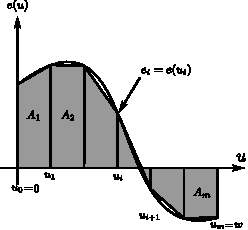
\includegraphics[width=3in]{figures_subgradient/integration_trapezoid.pdf}
 % integration_trapezoid.pdf: 119x111 pixel, 72dpi, 4.20x3.92 cm, bb=0 0 119 111
 \caption{Numerical intetegration of the function $e(u)$ by the trapezoid method for 1D $u$.}
 \label{fig:trapezoid}
\end{figure}


In this case, the interpolation function can change sign between sampling
points, so we have to be more careful with our integration.  For each sampling
interval between samples $i$ and $i+1$, there are multiple cases depending on
the signs of $e_i$ and $e_{i+1}$.  The cases with the same sign are
uninteresting; locally the $e_*$ values have the same effect on $f$ as they did
for the Rectangle Rule.  However, in the mixed sign case, the positive area
between the two interpolating points has a more intersting form:

%\begin{equation}\label{eqn:trapezoid_smoothing}
% \frac{e_i^2 + e_{i+1}^2}{2(\pm e_i \mp e_{i+1})}
%\end{equation}
%where the symbols $\pm$ and $\mp$ are the signs of $e_i$ and $e_{i+1}$, respectively (this just lets us use one expression for both an %increasing and a decreasing crossing). 


This expression is (at least locally) smooth in both $e_i$ and $e_{i+1}$.  Note
that unlike for the Rectangle Rule, we now have non-zero second partial
derivatives of $f$ with respect to $e_i$, and hopefully a meaningful Hessian of
$f$ with respect to $\x$.  {\em This could potentially lead to a Newton-like
minimization algorithm exhibiting second-order convergence}.  

% Discuss Continuous case

% Appending derivative of the functions in the optimization

% The non-smooth nature of the optimization problem is an artifact of our discretizatoin of the optimization problem

{\bf Extension to 2D domain} For face recognition applications, our $a_j$ and
$y$ correspond to images, i.e. they have a 2D domain.  Both the Rectangle Rule
and the Trapezoidal rule can be extended to these cases.  For the Rectangle
Rule, the extension is trivial, and leads to a sampled optimization problem of
the same form as for the 1D case.  

The 2D version of the Trapezoidal Rule is slightly more complex.  The image
plane is subdivided into triangular regions.  Within each region, the function
is approximated by a plane going through the graph of the function evaluated at
the three sampling points.  There are $2^3$ special cases: two with same sign,
and six with mixed sign.  For same sign cases there is just one volume to
compute, with mixed sign there are two.  

It may also be possible to make use of the 2D continuous nature of the data by
computing terms for the trapezoidal rule for all adjacent pairs of pixels in
both image directions.  Doing this would approximate the volume under the graph
of $|e|$ by the area of the volume's intersection with regularly spaced
vertical planes in both dimensions.  


{\bf Improving GPU Performance } There is reason to believe that algorithms
leveraging the above properties may be more amenable to efficient GPU
implementation.  One of the main factors governing GPU performance is the
number of arithmetic operations that are performed on data for each element
that has to be loaded into cache, a.k.a. arithmetic intensity.  GPU's typically
require an arithmetic intesity of about 7-15 floating point operations (FLOPS)
per load to achieve peak throughput.  

As a first example, consider the computation of a $m \times n$ matrix-vector
multiplication with $n$ small enough to fit into cache so that it need only be
loaded once.  A fused scalar multiply-add requires 1 FLOP, so the
multiplication will have an arithmetic intensity of about 1 FLOP/load.  Since
the Arithmetic Logic Units (ALU's) on the GPU can churn through the data faster
than it can be loaded, the time cost of the multiplication is roughly the cost
of loading $A$.  

As a second example, consider the computation of $A^T A$, again for $m \gg n$.
This can be computed as an $n \times n$ outer product of each row of A with
itself, plus an $n x n$ accumulation, for a total of $n \times n$ flops per row
of $A$.  Assume that this outer product fits into cache, so that we only have
to do $n$ loads per row of $A$.  This results in an arithmetic intensity of
$n$, resulting in much better usage of the ALU's of the GPU.

Since we have not been blessed with a problem that has an obvious
implementation with a very high arithmetic intensity in its formulation (and we
are not, at least for this part of the pipeline), we have two main avenues for
improving the efficiency of the algorithm on the GPU:

\begin{itemize}
\item Reduce the number of times we have to load the data arrays without
changing the arithmetic intensity.  First-order primal algorithms will have a
natural advantage over first-order primal-dual algorithms in terms of their
per-iteration cost, due to their relative simplicity.  However, it remains to
be seen if they will require fewer or less iterations to converge.

\item Reformulate the problem so that it has a higher arithmetic intensity.
For example, the extra computations for the trapezoidal rule may come almost
for free due to the data-local nature of the computation.  This may be
especially true for the triangle-mesh idea, since it falls very close to the
type of computations performed in a traditional graphics pipeline.

\end{itemize}

\section{L1 Minimization via Subgradient Descent} % TODO
{\bf Computing the steepest descent direction for rectangular integration }
%First order methods for solving extremely tall $\ell_1$ minimization problems are limited in speed primarily
%by their memory bandwidth requirements.  Furthermore, they require tuning and proper scaling of the data
%to ensure that they converge to the correct solution, and that the convergence occurs in a small number
%of iterations.  For this reason, these notes investigate algorithms that exhibit the following properties:
\begin{eqnarray}
\argmin{\x\in \Re^n} ||A \x - \bb||_1 \\
A \in \Re^{m \times n}\\
b \in \Re^m \\
\e = A \x - \bb \in \Re^m\\
f = ||\e||_1 \in \Re \\
\a_i = A(i,:) \in \Re^{n}\\
\end{eqnarray}

For simplicity we make the following assumptions on the problem matrices $A$ a $\bb$.
\begin{itemize}
\item $A$ and $\b$ are general arrays, i.e. we do not (yet) analyze special cases
where $A$ drops rank, there are duplicate rows, zero rows, etc.
\item $m$ is larger than $n$ to a degree that a $m \times n$ matrix-vector multiplication (gemv)
takes more time than inverting an $n\times n$ matrix.  
\end{itemize}

For some arbitrary point $\tilde\x$, we wish to compute a steepest descent
direction of $f$ and $\tilde\x$.  We begin by analyzing two cases.

In the first case, $\x$ does not lie on any attracting hyperplanes, i.e. $\e_i(\tilde\x)=0
\forall i$. In this case, the function is locally linear, and the gradient can be computed
by applying the appropriate sign change to each row of $A$, and then summing the rows of $A$:
\begin{eqnarray}
f_{local} &=& \sum_i |e_i(\tilde\x)| = \sign(\e(\tilde\x)) .* e(\tilde\x) \\
\nabla_x f_{local} &=& A^T * \sign(\e(\tilde\x)) \\
d &=& -A^T * \sign(\e(\tilde\x))
\end{eqnarray}
Note that once $\tilde\x$ is known, $d$ can be computed in a single pass through $A$.

The second special case analyzed is for the case where $\tilde\x$ lies on the intersection
of $n$ intersecting hyperplanes.  Without loss of generality, we reorder and partition the
matrices $A$ and $\bb$ such that the top $n$ rows correspond to the equations that are solved
with equality at $\tilde\x$:
\begin{eqnarray}
A = \left[\begin{array}{c}A_1 \\ A_2 \end{array}\right]\\
\bb = \left[\begin{array}{c}\bb_1 \\ \bb_2 \end{array}\right]\\
A_1 \in \Re^{n \times n} \\
A_2 \in \Re^{m-n \times n}
\end{eqnarray}
At $\tilde\x$, $\bb_1 = 0$.  Under our assumptions on $A$, $A_1$ is invertible.
We make the following state-dependent affine coordinate transformation:
\begin{eqnarray}
\hat\x &=& A_1\x - \bb_1 \\
\x &=& A_1^{-1} (\hat\x + \bb_1)
\end{eqnarray}
With this substitution,
\begin{eqnarray}
f(\hat\x) &=& ||\hat\x||_1 + ||A_2 A_1^{-1} (\hat\x + \bb_1) - \bb_2 ||_1 \\
&=& ||\hat\x||_1 + || (A_2 A_1^{-1}) \hat\x + (A_2 A_1^{-1} \bb_1 - \bb_2) ||_1 \\
&=& ||\hat\x||_1 + || \hat A \hat\x + \hat \bb ||_1
\end{eqnarray}
For infinitesimal $\hat\x$, the signs of the entries of the second term of $f$ will be
governed by the signs of the entries of $ \hat \bb = A_2 A_1^{-1} \bb_1 - \bb_2$.  
%Note: $A_1^{-1} \bb_1$ is the center of the linear
Note that due to our reordering of the rows, the entries of $\hat \bb$ are non-zero,
and the sign is well defined.
Therefore, $f$ locally reduces to:
\begin{eqnarray}
f(\hat\x) &=& ||\hat\x||_1 + \sign(\hat \bb)^T(\hat A \hat \x + \hat \bb) \\
&=& ||\hat\x||_1 + (\sign(\hat \bb)^T \hat A) \hat \x + (\sign(\hat \bb)^T  \hat \bb) \\
&=& ||\hat\x||_1 + \g^T \hat \x + ||\hat \bb||_1
\end{eqnarray}
For the purposes of deriving a descent direction, we can neglect the constant last term, leaving:
\begin{eqnarray}
f &=& ||\hat\x||_1 + \g^T \hat \x
\end{eqnarray}
This function has a stepest descent direction:
\begin{eqnarray}
\hat d &=& -\shrink(\g)
\end{eqnarray}
where the operator $\shrink(\x) = \sign(\x).*\max(|\x|-1,0)$ is the standard
soft thresholding operator. Mapping back to the original coordinate system and unrolling substitutions,
we have:
\begin{eqnarray}
\d &=& A_1^{-1} \hat \d \\
 &=& -A_1^{-1} \shrink(\g) \\
 &=& -A_1^{-1} \shrink(\hat A ^T \ \sign(\hat \bb)) \\
 &=& -A_1^{-1} \shrink(\hat A ^T \ \sign(A_2 A_1^{-1} \bb_1 - \bb_2)) \\
 &=& -A_1^{-1} \shrink(A_1^{-T}A_2^T \sign(A_2 A_1^{-1} \bb_1 - \bb_2))
\end{eqnarray}
Unfortunately, while $\hat \d$ is the steepest descent direction for the optimization in transformed coordinates,
$\d$ is in general not the steepest descent direction for the original problem.  
{\em What if only some rows of $e_1$ are zero?}

{\bf Conclusion } The special nature of the data may be able to improve the design of a search algorithm in the following ways:
\begin{enumerate}
\item For $m \gg n$, we can get away with a trivial choice of subgradient as a descent direction.
\item There will likely exist monotonic runs in $\frac{y_i}{a_i}$.  This significantly reduces the cost of a sort operation, making it feasible to compute an optimal step size for a given descent direction.  
\item It may be possible to compute a good approximation to the Hessian of the continuous optimization problem, resulting in an algorithm requiring far fewer iterations to convergence.  
\item The nature of the above computations may be significantly more amenable to efficient GPU implementation due to their simplicity and/or higher arithmetic intensity.
\end{enumerate}

\end{document}
